\chapter{Mouse Behaviour in Complex VR Tasks}
\label{chapterlabel3}

\section{Can Mice Learn Visually Complex Navigation Task?}
 Many recent studies in mouse VR navigation tasks use tall and large visual landmarks which can be seen and distinguished from far away with floor patterns as only background. In the experiment design I use, it presents the challenge to the mouse that it needs to differentiate sets of identical landmarks in grayscale and the well-controlled white noise gray background. Compared to primates, cats, birds, mice have low acuity vision. One may argue that mouse cannot differentiate such detailed visual landmarks in a VR setting to form clear representations of the space. In Saleem et al. 2018, they've trained the mice to actively lick for a reward associated to one of the identical plaid landmarks spaced at 20cm in a 100 cm corridor. Here in one of the environment, I use a familiar set of landmarks but with an additional cue landmark at the start with extension of extra 40 cm. Further to that, the VR corridor is constrained to only show 21cm ahead of the mouse rather than the full view ahead. This method prevents the mouse knowing what landmarks are ahead until it passes the current landmark and it is different from the conventional VR task particularly in studies on hippocampus and entorhinal cortices. Therefore, it can be perceptually more challenging to distinguish one visual landmark and 2 sets of identical visual landmarks in 100 cm space. In addition, in the recording period, there would be an extra environment introduced to the animal and the novel environment contains one of the same set of landmarks, that is, the plaids, and the mouse is required to distinguish the two environments are different. In this chapter, I will show mice can learn visually complex navigation tasks.
 \begin{figure}
    \centering
    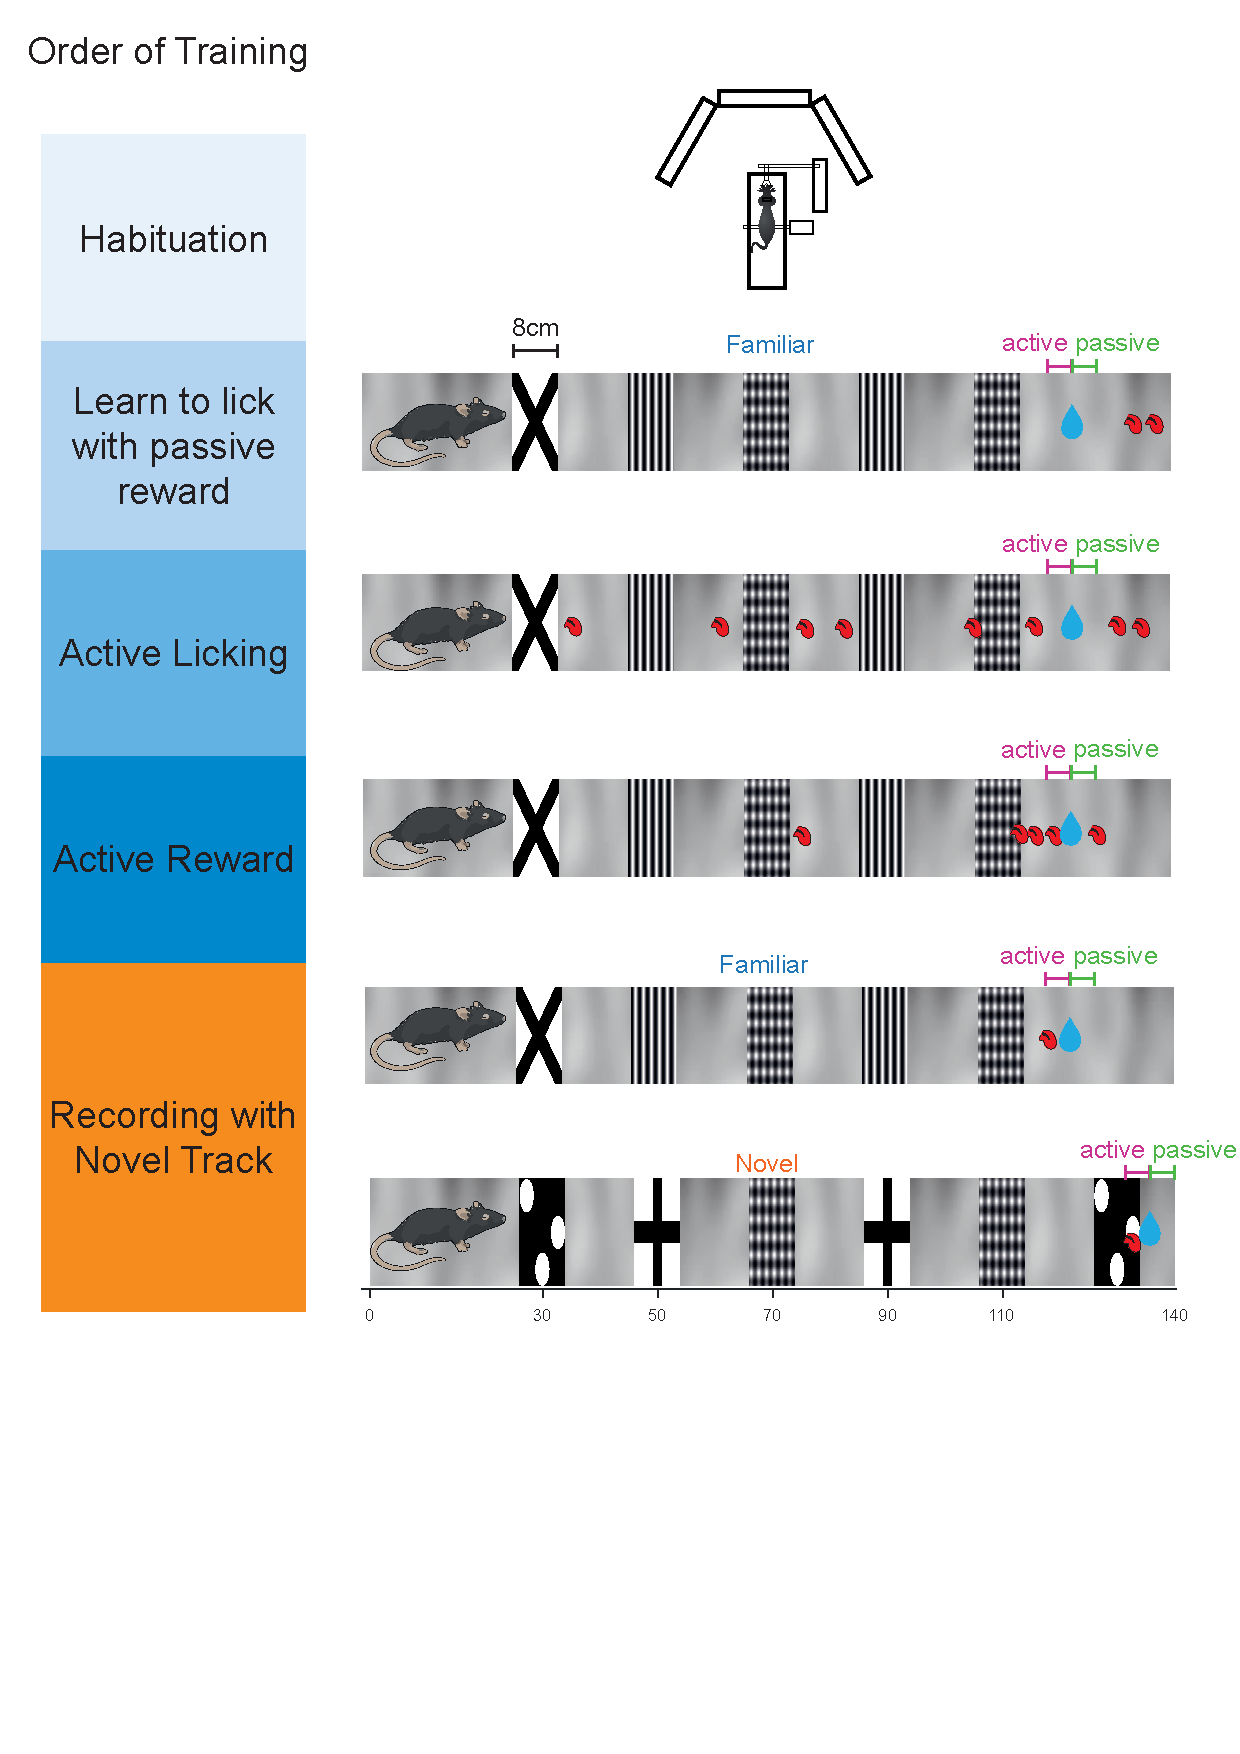
\includegraphics[width=1\linewidth]{figures//Chapter 3 Behaviour//Thesis Figures//figure_PDFs/fig1_behaviour_training.pdf}
    \caption{Training stages from habituation to recordings. }
\medskip
\small
The illustration gives examples of licking behaviour over stages of training. In early stage, the mouse can only lick after a passive reward is given. After habituation to the reward and licking, the mouse can lick actively everywhere in the VR. Once learned, the active licking is more likely to be around reward zone. Once the mouse is ready, it undergoes craniotomy surgery and the ephys recordings start with the introduction of novel VR environment.
    \label{fig:overall training stages}
\end{figure}

\section{Methods}
\subsection{Animal Training Stage}
Duration of learning the task to perform stable active reward trials can vary between mice. To avoid any bias in further analysis, the learning is divided into early, mid, late stages by taking first 1/3, mid 1/3 and late 1/3 sessions of the total number of sessions for a mouse.


\subsection{Lap Type Categorisation}
In further analysis of learning behaviour, each lap across sessions is classified as one of the six lap types. Each lap in session data is already categorised as passive or active or aborted. They further categorised by the positions of licking events during the lap. 
Passive laps are divided into (1) passive and no licking if no licking happens before the reward is given and (2) passive licking if licking occurred before reward is given. 
Active laps are divided by whether the lap has licking only before the active reward is given within 10cm: if yes, it is classified as active precise and if no, it is classified as active with licking. 
Aborted laps are laps aborted due to either 1) staying on the same lap for more than 90 seconds; or 2) licked more than the lick threshold set at the time ( in early training, the licking threshold is 20 times and in late training, the licking threshold slowly goes from 15 times to 10 times). If there is no licking at all in an aborted lap, the lap is classified as aborted with no licking and any other aborted lap is classified as aborted with licking.

\subsection{Transition State and Preference Matrix}
All laps across mice are pooled together and the overall probability of a lap type occurring is the total number of the lap type divided by total number of laps \(\pi_j = P(X_t = j) = \frac{\text{Total count of state } j}{\text{Total number of laps}}\). For the interest of further analysis of how likely a lap type transitions into one of the lap types in the next lap, a transition matrix calculated by \(P_{ij} = P(X_{t+1} = j \mid X_t = i) = \frac{\text{Count of } i \to j \text{ transitions}}{\text{Total count of transitions from } i}\) where i is the current lap and j is the next lap. Any last lap of the session is excluded from i. A preference matrix is calculated to observe which lap type is favoured by a certain lap type based on transition matrix: \(M_{ij} = \frac{P_{ij}}{\pi_j} = \frac{P(X_{t+1} = j \mid X_t = i)}{P(X_t = j)}\). For visualisation of the positive being favoured and negative being disliked, a log 10 is applied to the preference matrix.

For comparing preference matrices at each learning stage, the preference matrices are divided by the same overall probability across sessions and mice.

\begin{figure}
    \centering
    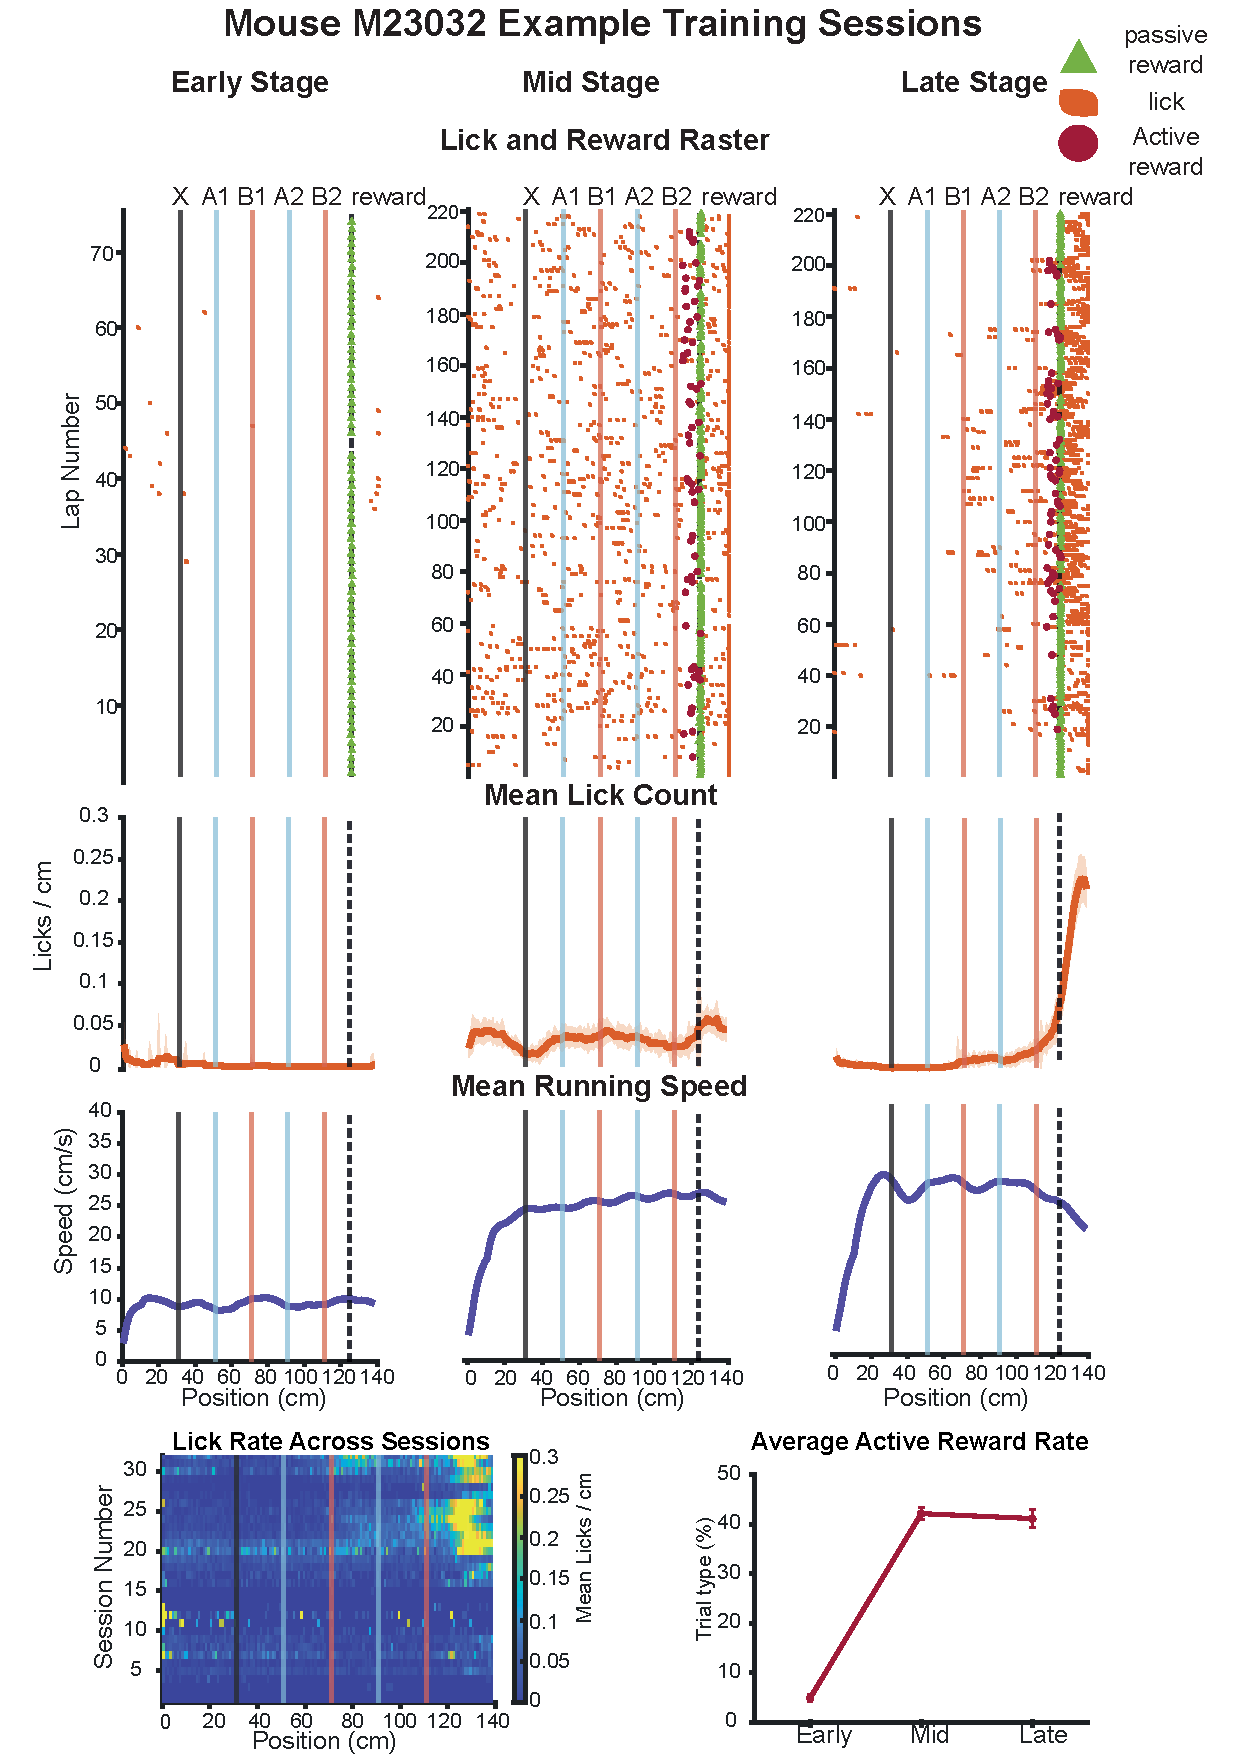
\includegraphics[width=1\linewidth]{figures//Chapter 3 Behaviour//Thesis Figures//figure_PDFs/fig2_example_sessions.pdf}
    \caption{Example training sessions at different stages of the training.}
\medskip
\small
 The three examples from mouse M23032 are each from early, mid, late stages of the training. \textbf{A)} Raster plots of licking, active rewards and passive rewards events. Green triangle is passive reward, yellow round object is mouse licking detected, red circle is active rewards. Y axis is the number of laps in the session and x axis is the position of the mouse. \textbf{B)} The average lick count at each position across laps in the session. Y axis is the mean lick count/cm and the x axis is the position. \textbf{C)} Average running speed at each position across laps in each session. The y axis is the speed (cm/s) and x axis is the position. \textbf{D)} The heatmap of overall mean lick count across sessions. Y axis is the session number and x axis is mouse position. The licking distribution slowly evolves into more active lickings around reward zone over learning. \textbf{E)} Average percentages of active reward in early, mid, late sessions. 
    \label{fig:example training sessions}
\end{figure}



\begin{figure}
    \centering
    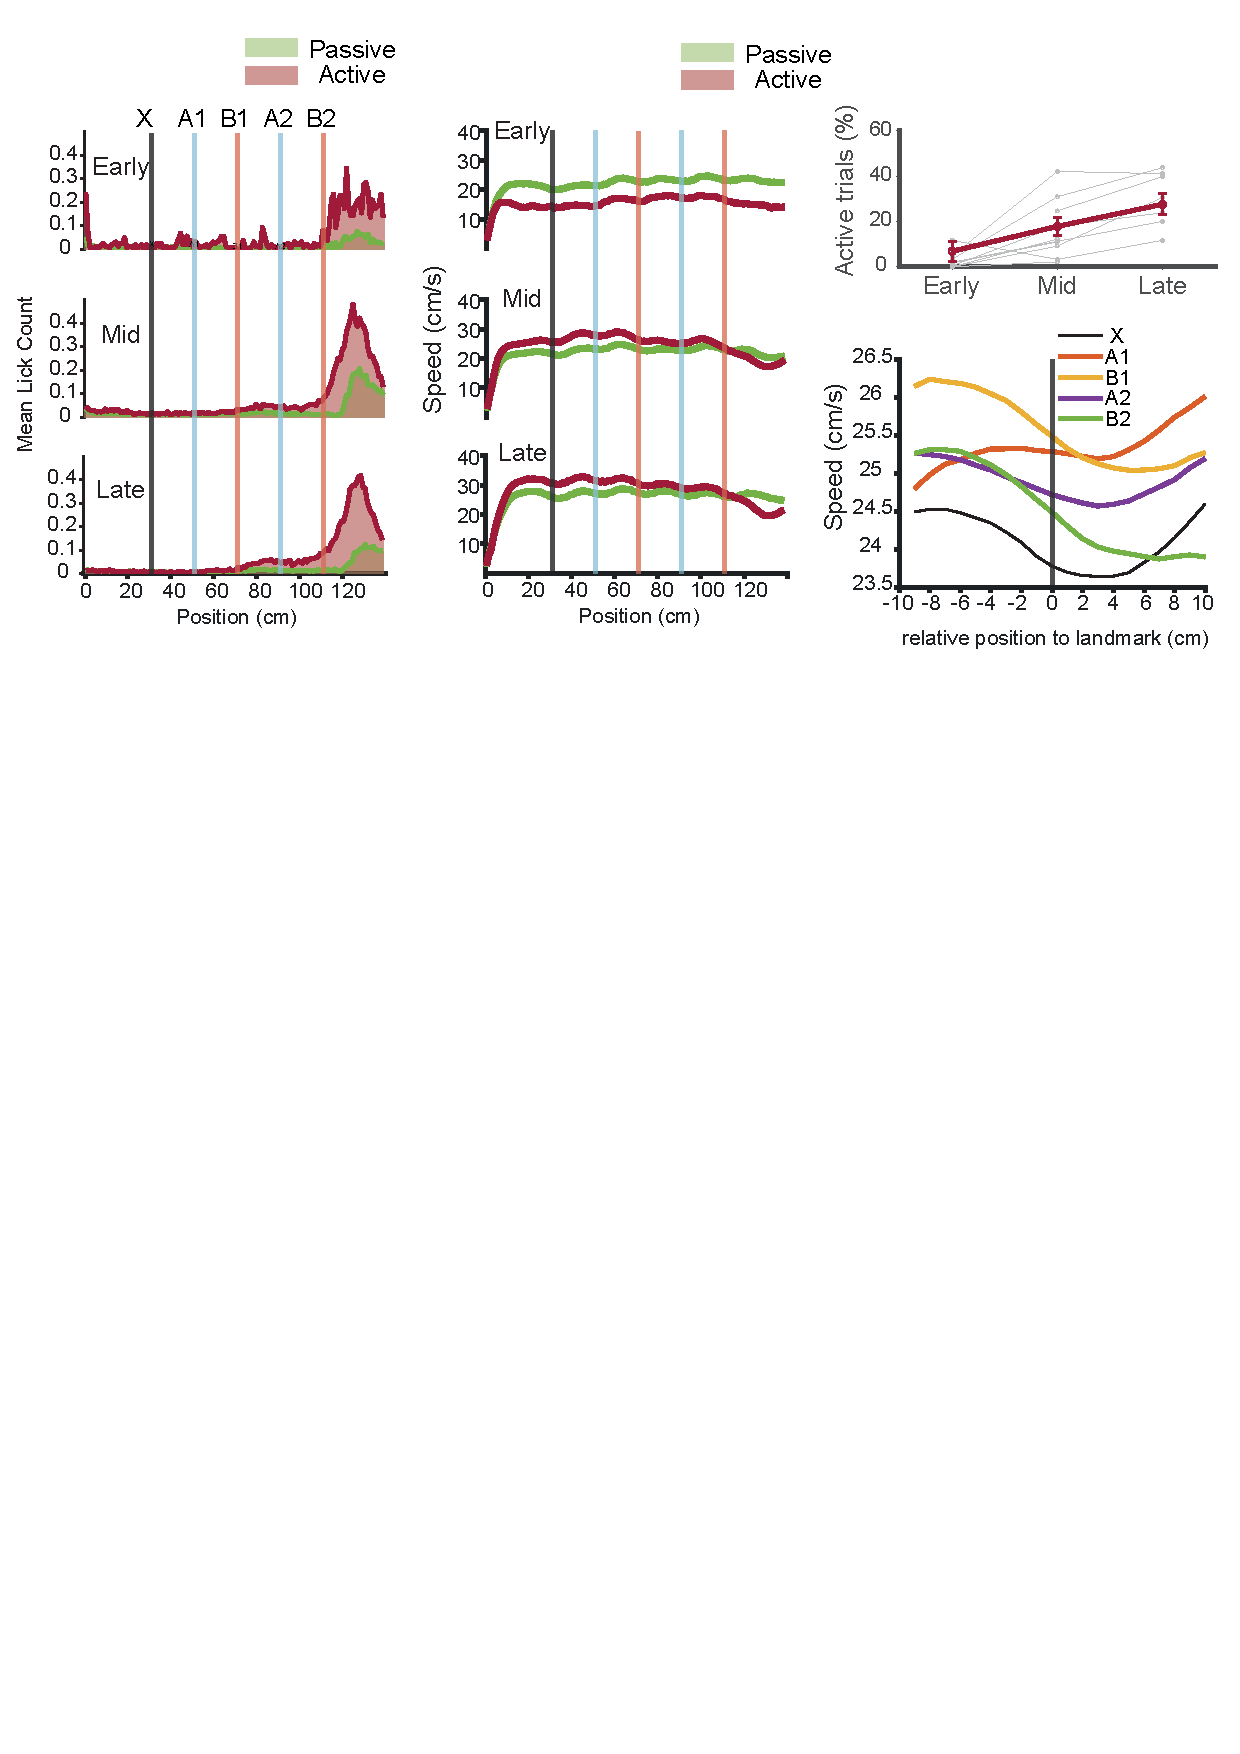
\includegraphics[width=1\linewidth]{figures//Chapter 3 Behaviour//Thesis Figures//figure_PDFs/fig3_behavioural_learning_summary.pdf}
    \caption{Behavioural Training Summary. }
\medskip
\small
Summaries of licking, running, and active reward rate across mice from early to late stage training. \textbf{A)} Average licking counts across mice from early to late training stages. Red is active reward trials and green is passive reward trials. \textbf{B)} Average running speed across mice along the VR corridor. Red is active reward trials and green is passive reward trials. \textbf{C)} Average active reward trial percentages from early to late stages and gray dots and lines are individual mice.
    \label{fig:training behaviour summary}
\end{figure}

\section{Results}
\subsection{Mice Can Perform Active Behaviour in a Complex VR Setting}


In Chapter 2 method of behavioural training, a detailed training protocol is described. Here in Fig 3.1, the sequence of the learning is described. After habituation, the mouse runs through the VR environments with a passive reward given. Over days, the mouse learns how to lick in the lickport and start active licking along the corridor. With the active licking, the mouse can trigger the active rewards themself which is within 5 cm before the reward zone mark. After learning where the reward zone is, the mouse commonly reduces licking at other locations and lick more frequently just before the reward zone but sometimes after the first plaid which can be confused between the two plaids. Overall, there are 14 mice trained and they all successfully performed ative licking and active reward laps. 2 out of the 14 mice were trained with the opposite track which is the novel track for the other 12 mice. A quantitative summary of the active behaviour learning will be presented.

Mouse has very different behaviour at early, mid and late stages of the training sessions in terms of licking, running and performance. In Fig 3.2, three example sessions from each stage of M23032 learning the task are shown. The top row is the lick event and reward raster at all laps. In early stage training session, the animal licks very little and rewards are all passive rewards. The licks at the start of laps are usually when the mouse realized there is reward much later than the reward delivery time during the start of the next lap already. In Fig 3.2B, this early session has near zero mean lick count across positions in the VR. In addition, the average running speed of the mouse is very slow in Fig 3.2C. In contrast, the mid and late stages have much higher overall ick counts across positions and running speed across trials. However, the distributions of the licking and running are different. First, in mid stage, the licking events are all over positions across the VR in Fig 3.2A and the mean lick counts are more evenly distributed along positions in Fig 3.2B. Whereas in late stage, the lickings are more located at later part of the VR and particularly high when near the reward zone in both Fig 3.2A and Fig 3.2B. The licking distribution has a small bump and a large bump in average licking count distribution for late stage in Fig 3.2B. Further to mean running speed in Fig 3.2C, the mouse has similar running speed in both mid and late stages but there's more slowing down after the mouse reaches the B1 and B2 which agrees with previous VR studies that animals tend to slow down and perform predictive licking to the reward justs before reward location. Overall this indicates that the mouse learns association of the B landmarks to the rewards and sometimes can mistaken B1 and B2 but overall the licking is more centralised between the B2 and reward zone. More than just these three example sessions, Fig 3.2D shows the average licking across positions in all sessions chronologically ordered. Around 1-15 sessions, random licking along position developed. From 15 to 30 sessions, the mouse slowly changed the licking strategy from licking randomly to just the Bs and reward zone. In Fig 3.2E, the average active reward rate is shown across stages of learning and the mouse performs similar active reward rate between mid and late stages. But the licking and running behaviour show that the mouse shows more precise active reward behaviour in the later stage of the training.

Across mice, the licking distribution, running behaviour and active reward rate are similar at each stage of learning. In Fig 3.3, averages across mice are shown in terms of licking, running and active reward rates. Further to that, the laps are divided into passive and active laps. First, for mean lick count in Fig 3.3A, all mice show random licking along positions in both active and passive laps and there are more licking in both mid and late stages. In mid stage, the mouse licks more along all positions but the mouse licks more in the later part of the VR after B1. Further to that, both stages show a small bump at B1 and a large bump between B2 and reward zone in active laps and a small bump at B1 is also present in passive laps but not much licking before reward zone. In terms of running in Fig 3.3B, In mid and late stages' active laps, there's an obvious trend of slowing down before reward zone as well. For all animals, there is a trend of increase in active reward rate over learning in Fig 3.3C. In all these summaries, two mice that were trained in the other track are included.





\begin{figure}
    \centering
    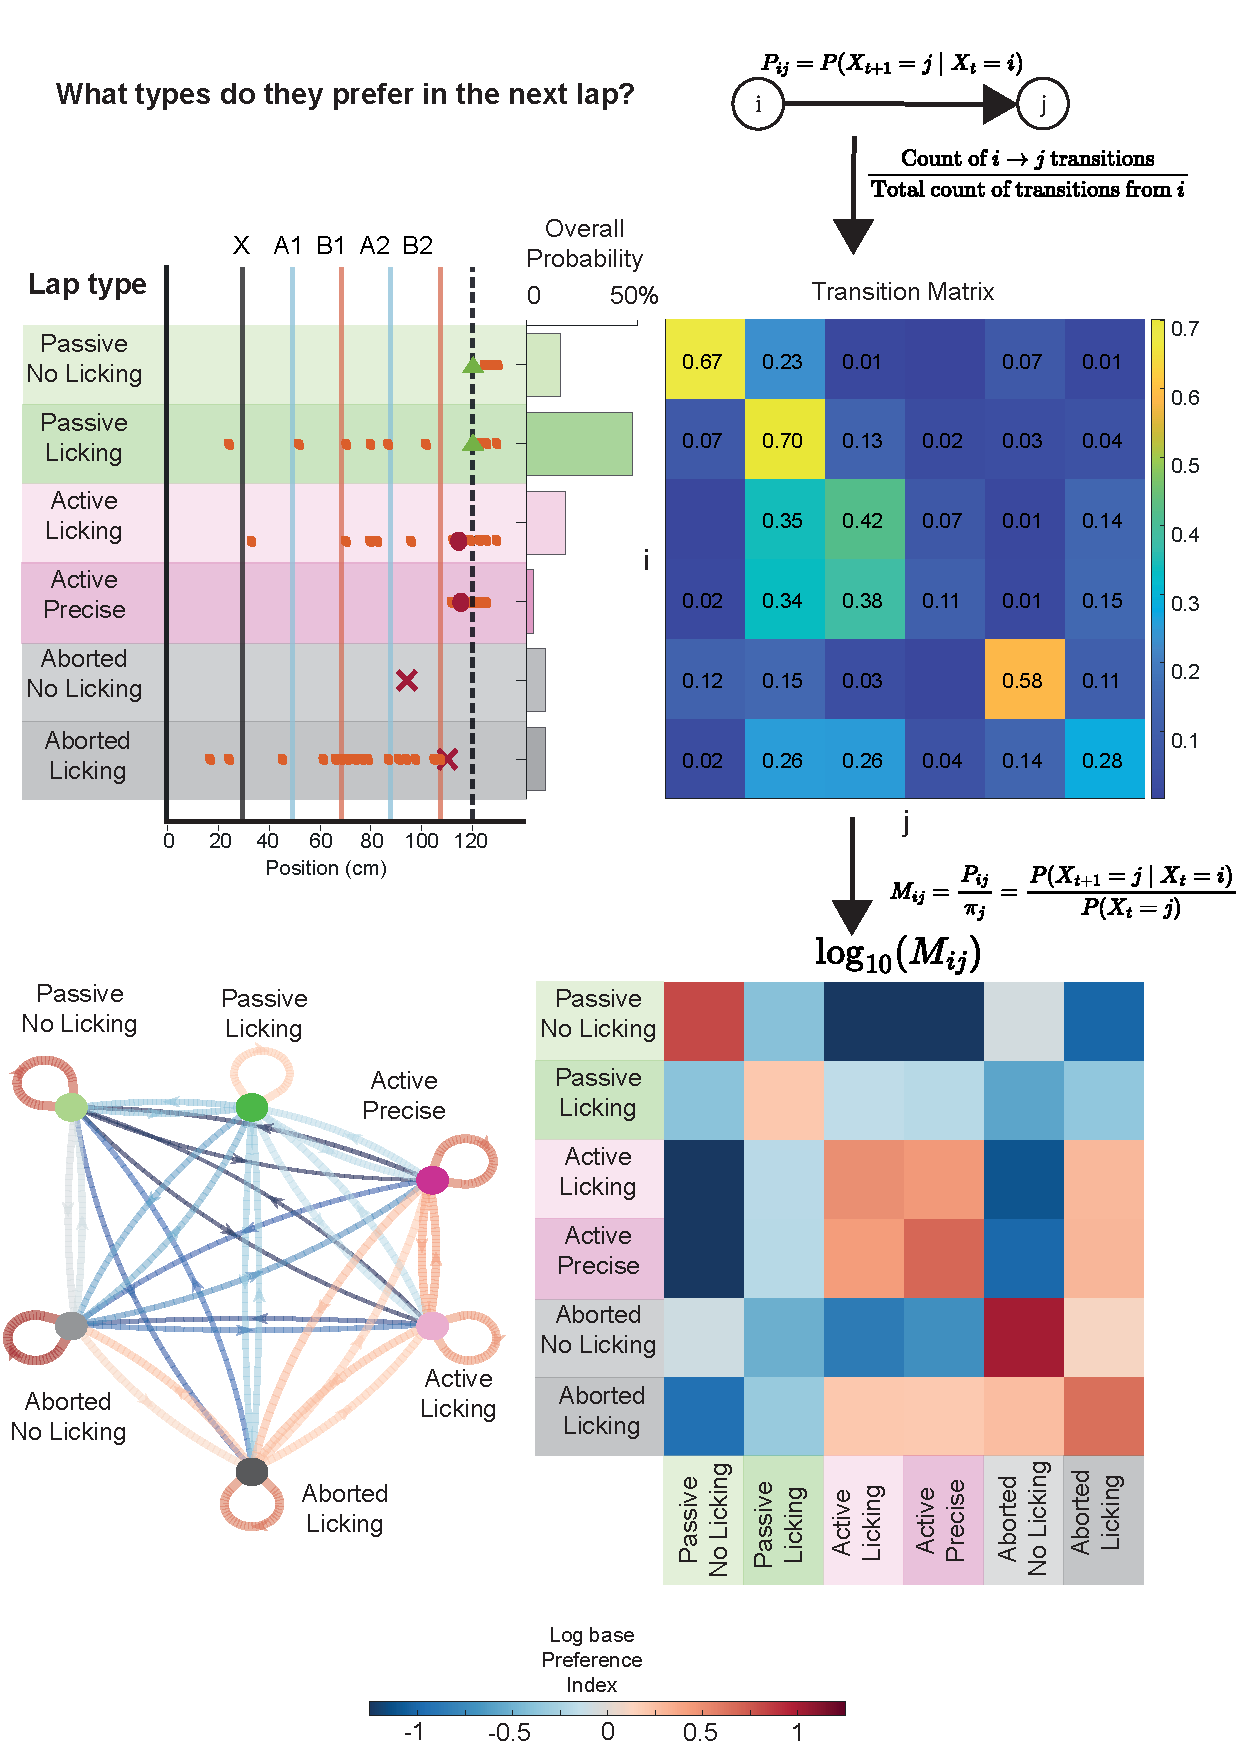
\includegraphics[width=1\linewidth]{figures//Chapter 3 Behaviour//Thesis Figures//figure_PDFs/fig4_transition_matrix.pdf}
    \caption{Laps of VR can be categorised into various types and they have preferences of which type to transition into.}

\medskip
\small
Demonstration of lap type categories, their transition matrix and their preference of transition which raises a question: when a lap type happens at lap i, does the animal prefer transitioning into a particular lap type at the next lap j? \textbf{A)} Each lap in the VR is categorised as one of six lap types. This panel demonstrates examples of each lap type and corresponding overall probability of lap type occuring next to the example. \textbf{B)} Illustration of how probabilities of transition state are calculated and an overall transition state matrix. \textbf{C)} Illustration of how to calculate preference index by dividing transition state probability over overall probability. Log likelihood of the preference can represent the direction of preferences well. On the left is the graph of the preference matrix and on the right is the preference matrix in log likelihood. 
    \label{fig:how to preference matrix}
\end{figure}

\subsection{Lap Types Have Transition Preferences}
In above results, the mice are shown to learn the task to perform active reward acquisition at a reward zone overall. However, during learning, the mice can have lap by lap variability in terms of behaviour and this variability can reveal the animal's current behavioural state and how these behavioural states can change over learning. In order to capture the variability in laps, the laps are further classified into 6 types from just active and passive laps based on the licking behaviour. In Fig 3.4A, examples of each lap type are shown and their corresponding overall probability across sessions and mice. Both passive and aborted laps are simply divided into with or without licking before reward is given. For active laps, they are classified by if the mouse can perform an active reward lap precisely or not which means if the mouse only licked within 10 cm before active reward is obtained. Passive with licking is the most common lap type, and both active with licking and passive with no licking are second highest. The rest are relatively low probability overall. 

Do these lap types have relations to each other? A transition matrix is calculated to compare how likely a lap type X transitions into a lap type Y from lap i to lap j (Fig 3.4B). To normalise the imbalanced overall probability of lap types, a preference matrix is calculated by dividing the transition matrix over the overall probability of the lap types in next lap j. In Fig 3.4C, an overall preference matrix is shown with log 10 based likelihood indicating that the lap type X prefers lap type Y if log likelihood is above 0, and it does not prefer lap type Y if it is below 0. Next to the matrix, it is a graph plot of the matrix to visualise the relationship between lap types. First, in both diagonal of the matrix and the self loop of the graph, lap types prefer transitioning into themselves. Second, active lap types and aborted with licking have high preferences between each other forming a small hub of lap type transitions. Third, passive with no licking prefers itself highly but have relatively higher likelihood to transition into either aborted with no licking which means mouse is immobile for a long duration or passive with licking which means the mouse starts licking and passive with licking will further transition into active lap types. Thus, when animal is not engaged and starts transitioning back to active behaviour, it will first more likely transition into passive with licking and then transition to active reward lap types rather than transition to active reward lap types directly. Taken together, this shows a hint of 3 major behavioural states of the mouse: inactive - staying within the hub of passive with no licking and aborted with no licking, active licking but low performance - staying within passive with licking, and engaged with active rewards - staying within the hub of  active precise, active with licking and aborted with licking. The mice prefer to staying within the current behavioural states. But how are they the same over learning?

Learning the active task changes the lap type preference strength. In early stage, the self-loop strength within the lap types is strong (Fig 3.5). From mid to late stage, the self-loop strength within the 6 lap types becomes weaker (Fig 3.5). Overall, the transition preference becomes weaker in the late stage as well (Fig 3.5) which indicates that there are more transitions between all lap types particularly between passive with licking and active lap types. However, the behavioural state of passive with no licking and aborted with no licking prefers staying within itself more in the late stage. 





\begin{figure}
    \centering
    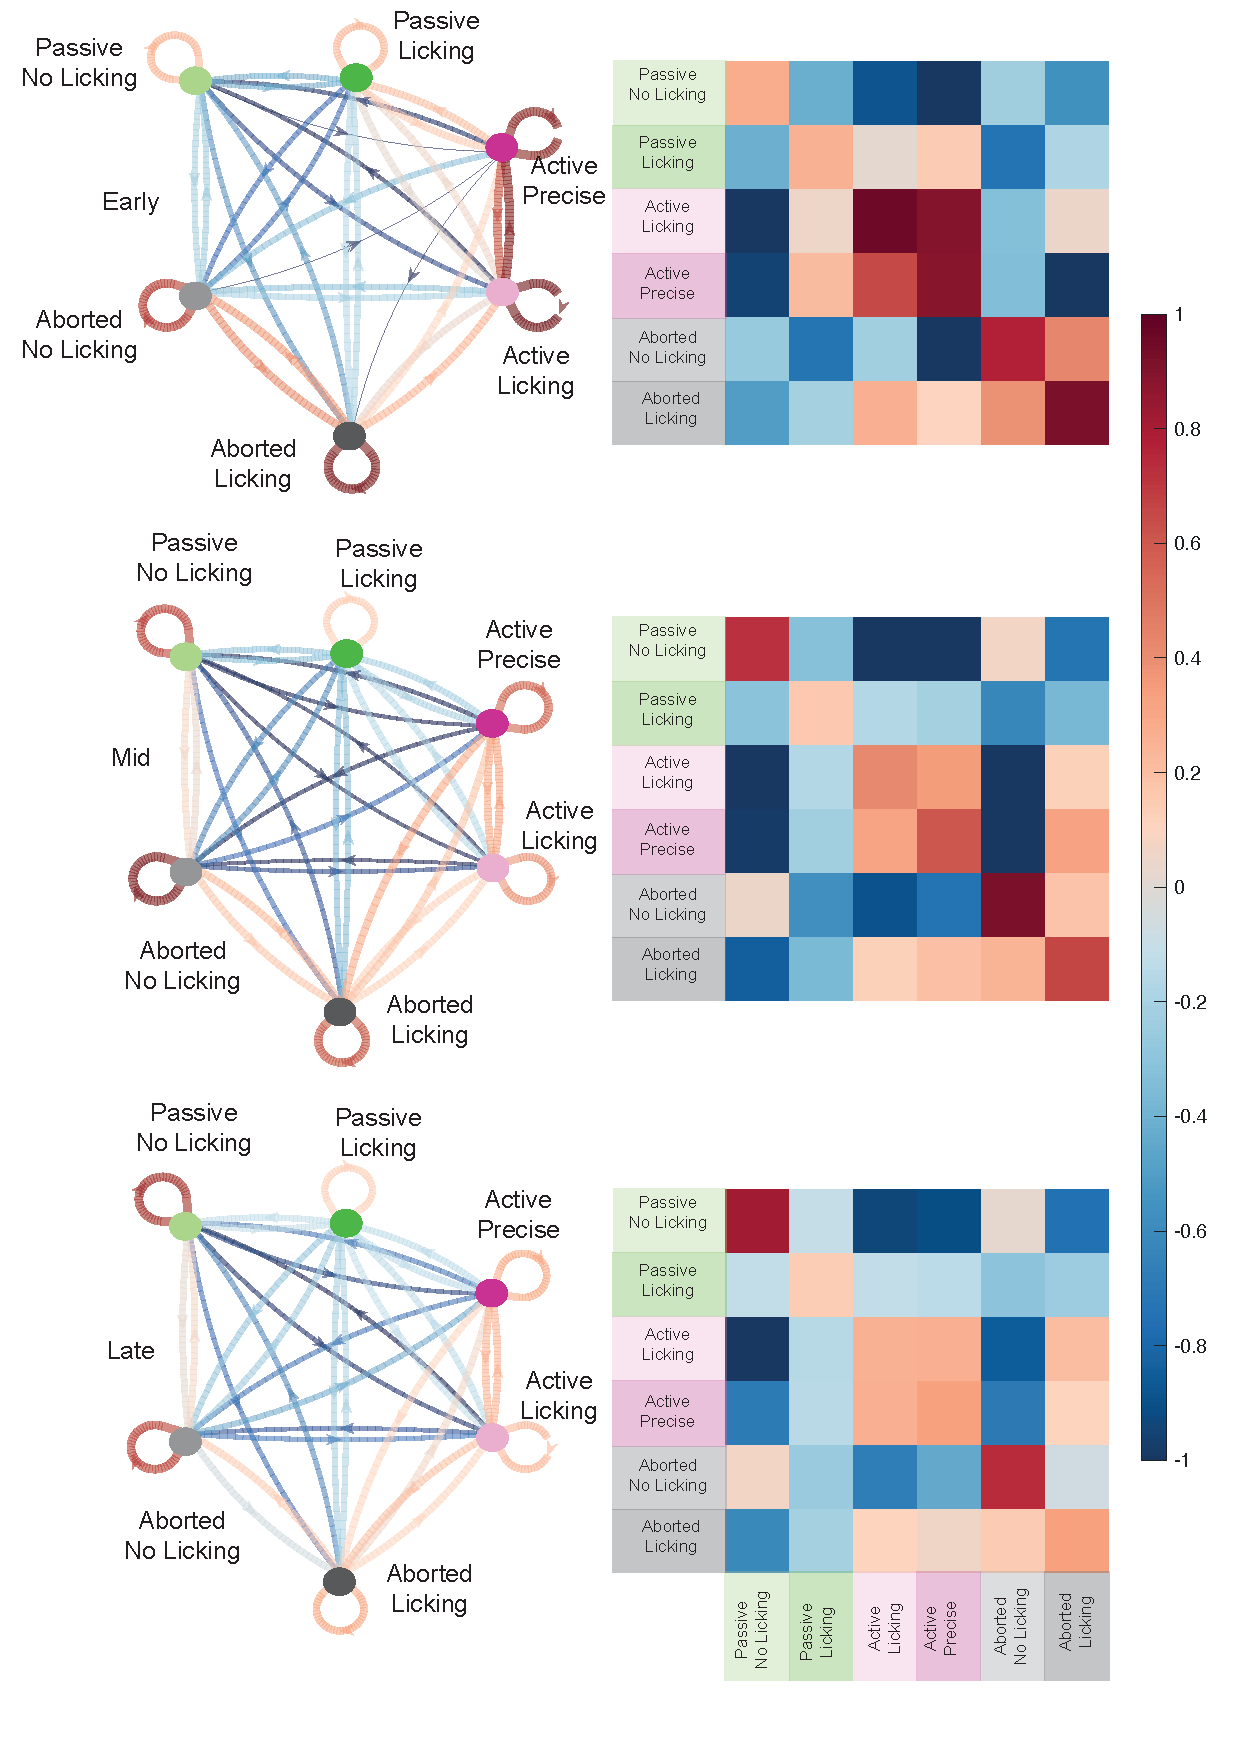
\includegraphics[width=1\linewidth]{figures//Chapter 3 Behaviour//Thesis Figures//figure_PDFs/fig5_preference_index_each_stage.pdf}
    \caption{Preference matrix for lap types over stages of training.}
\medskip
\small
Illustration of preference matrix over lap type at early, mid, and late stages of the training across mice. The preference matrix is presented as both graph and matrix itself for convenient interpretation.
    \label{fig:preference matrices over learning}
\end{figure}





\subsection{Mice Can Distinguish A Novel Environment from Familiar Environment Behaviourally}
\begin{figure}
    \centering
    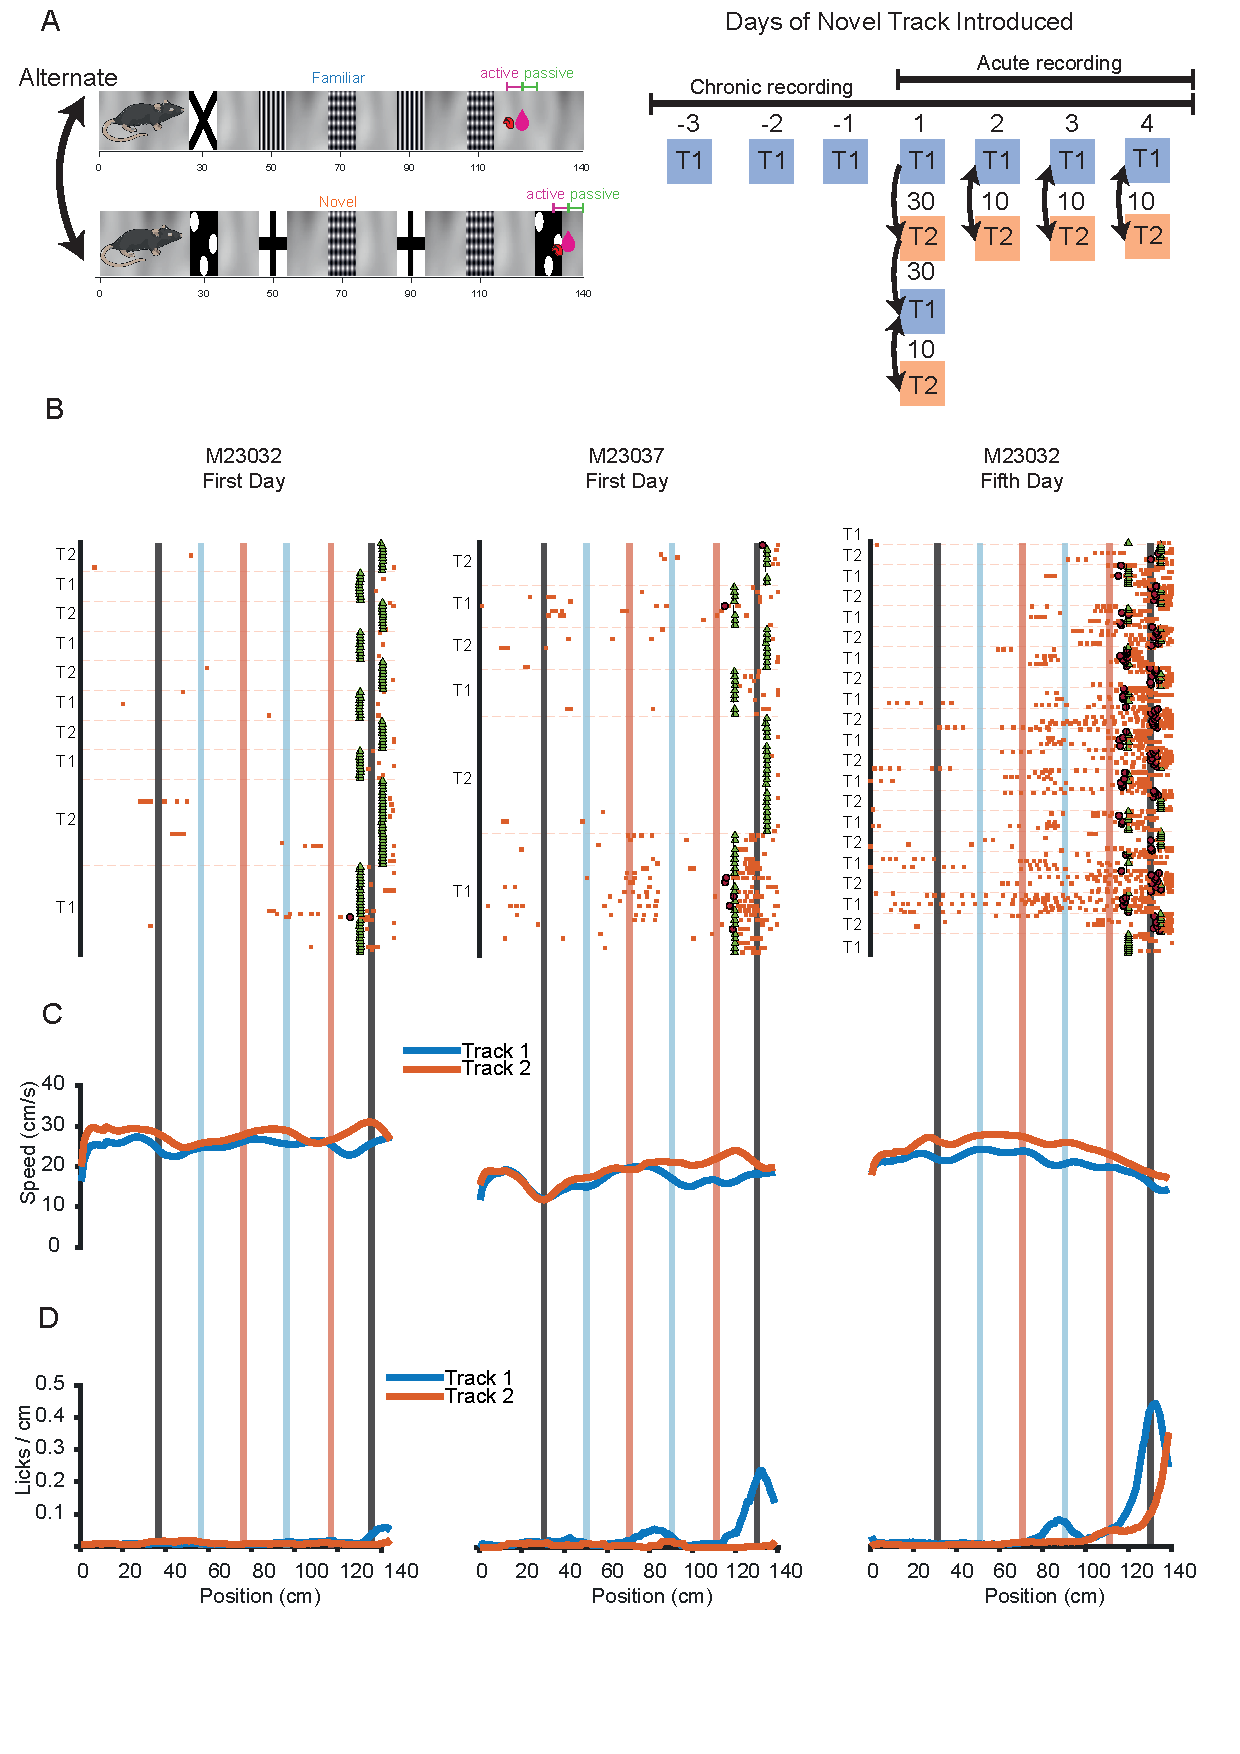
\includegraphics[width=1\linewidth]{figures//Chapter 3 Behaviour//Thesis Figures//figure_PDFs/fig6_novel_track_behaviour_examples.pdf}
    \caption{Mice adapt their behaviour when a novel environment is introduced.}

\medskip
\small
Examples of recording sessions behaviour when a novel environment is introduced. \textbf{A)} Demonstration of the experiment design and the timeline for when novel environment is introduced in recordings. \textbf{B)} Example raster plots of three sessions from recordings. Some sessions have poor active licking behaviour and the third example session shows high active licking behaviour in both environments. \textbf{C)} Average running speed in each session. Blue color is track 1 and red color is track 2. Track 2 is the novel environment. On average, the running behaviour is similar and much more different at the later part of the two environments. \textbf{D)}  Average lick count in each session. Track 1 is blue and track 2 is red orange. The licking distribution is different between the two tracks.  
    \label{fig:placeholder}
\end{figure}
After training and craniotomy, the animal is introduced to a novel environment with electrophysiology recordings. The novel environment is introduced after 30 laps of familiar on the first novel day. The timeline is described as in Fig 3.6A that the animal is introduced to the novel environment on first day of acute recordings or 3-5 days after chronic recordings. After introduction of the novel environment for 30 laps, the two environments always alternate every 10 laps and it is the same 10 lap alternation in the following days. The novel environment contains the same plaid landmarks at the exact locations and the other landmarks are at the same locations but swapped with other visual patterns. A sixth cue landmark at 130 cm same as the first one is added and a reward zone is moved to 135 cm from 120 cm in the familiar environment after the sixth landmark. These additions are implemented to make the mouse distinguish the two environments. Due to long duration of the craniotomy surgery, the mouse might not recover well on first 1-3 days of the acute recordings and can behave badly even in the familiar environment. Here three example sessions with bad and good behaviour are shown to illustrate how the mice can behave different to the two environments (Fig 3.6B - D).

The licking distribution and running pattern are different in the two environments, and the mice can learn to obtain active rewards at different reward zones in the two environments. In Fig 3.6B, first and third sessions are the same mice from first and fifth days and the second session is from another mouse from its first day. The lick and reward raster plots start the session from the bottom to top. The first session is a bad behaviour day that the mouse only manages to obtain one active trial. However, in the second session, the mouse also has relatively bad behaviour but it can obtain a few active rewards and managed to obtain active reward of the novel environment at the end of the session (Fig 3.6B). In the third session which is the fifth day already, the mouse can obtain high amount of active rewards reaching to about 60\% and can lick differently in the two environments. By comparing the running pattern, all sessions appear to have very different running pattern in the two environments especially in the later part and the third session actually has the two environments' running patterns more similar as the mouse is very familiar with both environments (Fig 3.6C). In Fig 3.6D, the licking behaviour is correlated with how good the animal behaviour is and the first session has licking mostly after reward is given. In the good licking sessions, the licking count distributions in the familiar environment are similar as the training stage that there is a small bump of high licks at B1 and a large bump between B2 and reward zone, whereas the novel environment has the licking bump skewed towards the new reward zone. (Fig 3.6D). Overall, the mice behave differently in the two environments and over more days, the behaviour becomes better.


\section{Discussion}
In this chapter, the animal behavioural training is examined with quantitative methods. By these methods, the trained mice can behave better to obtain an active reward in a visually-complex VR environment after learning. In the late stage, the mouse can control their licking and running better to obtain the active and even the passive rewards without over-licking. Due to the cognitive difficulty of tracking identical landmarks, the mice do not have very high active reward rates exceeding 50\% at the end of training. However, the passive reward laps also show that the mice can slow down to the reward zone and control their licking which indicate they are very familiar with the environment. In addition, this is reflected by that observation passive with licking lap type acts as an intermediate state between engagement and disengagement. In the analysis of the transition states between lap types, the preferences of lap types reveal these hubs of behavioural states and give insights on how to use them to compare if the mouse learned the task. In addition, this lays a foundation to model animal behaviour in a VR environment. Unfortunately, due to time limit, this method is not applied to the novel environment which might have very different dynamics from introduction to novel environment to becoming familiar with the novel environment. However, in the last part of the chapter results, it is shown that the mice are able to distinguish the two environment behaviourally and the future lap type preference analysis will make it clearer to use the novel vs familiar behaviour to analyse neural data. Further to that, videos of the animals were recorded but time limit makes it impossible to analyse them yet. The videos contain the animal's pupil, face and paw tracking which can provide more information about if the animal's learning stages can be predicted by these variables and the animal's reactions to changing of the two environments. In the next chapter, I will discuss how neurons in V1 respond differently to the two environments rather than the behaviour. 

